This chapter presents the implementations\footnote{This is an open source project. One can find the essential software implementations on our GitLab page at \url{https://gitlab.tue.nl/20181234/brewery_dt}, as well as the overview of equipment in Appendix \ref{apd:workbench}.} of \textbf{S1} (Production Prediction) and \textbf{S2} (Production Control) mentioned in Chapter \ref{ch:methodology}, using each of the three selected frameworks in order to showcase the possibilities of integration and orchestration approaches. As explained in Section \ref{sec:5dbrewery}, \textbf{S3} and \textbf{S4} are not implemented in this project.

Despite the influence of bio-chemistry theme in our case study, we choose to convert all VE models to FMUs over the CAPE-OPEN standard for the sake of generalizing the approach so they can extend to other domains. As FMI is more inclusive to a wider range of models for integration.

\section{Production Prediction (S1) demonstrations}\label{sec:s1demo}
In \textbf{S1}, the DT collects readings from the three sensor devices of the PE. The scanning period is set to five minutes; we consider this frequency adequate for monitoring the slow variations of the process. After merging the monitoring data, the models of the VE will be invoked to compute the final predicted wort temperature using the given data. Besides, the three chemistry models (see also Section \ref{sec:5dbrewery}) have data dependency to one another.

\subsection{S1 in TwinOps} \label{sec:s1twop}
Figure \ref{fig:s1_twop_workflow} shows the technologies that compose the building blocks of the TwinOps workflow:

\begin{figure}[hbt!]
  \centering
  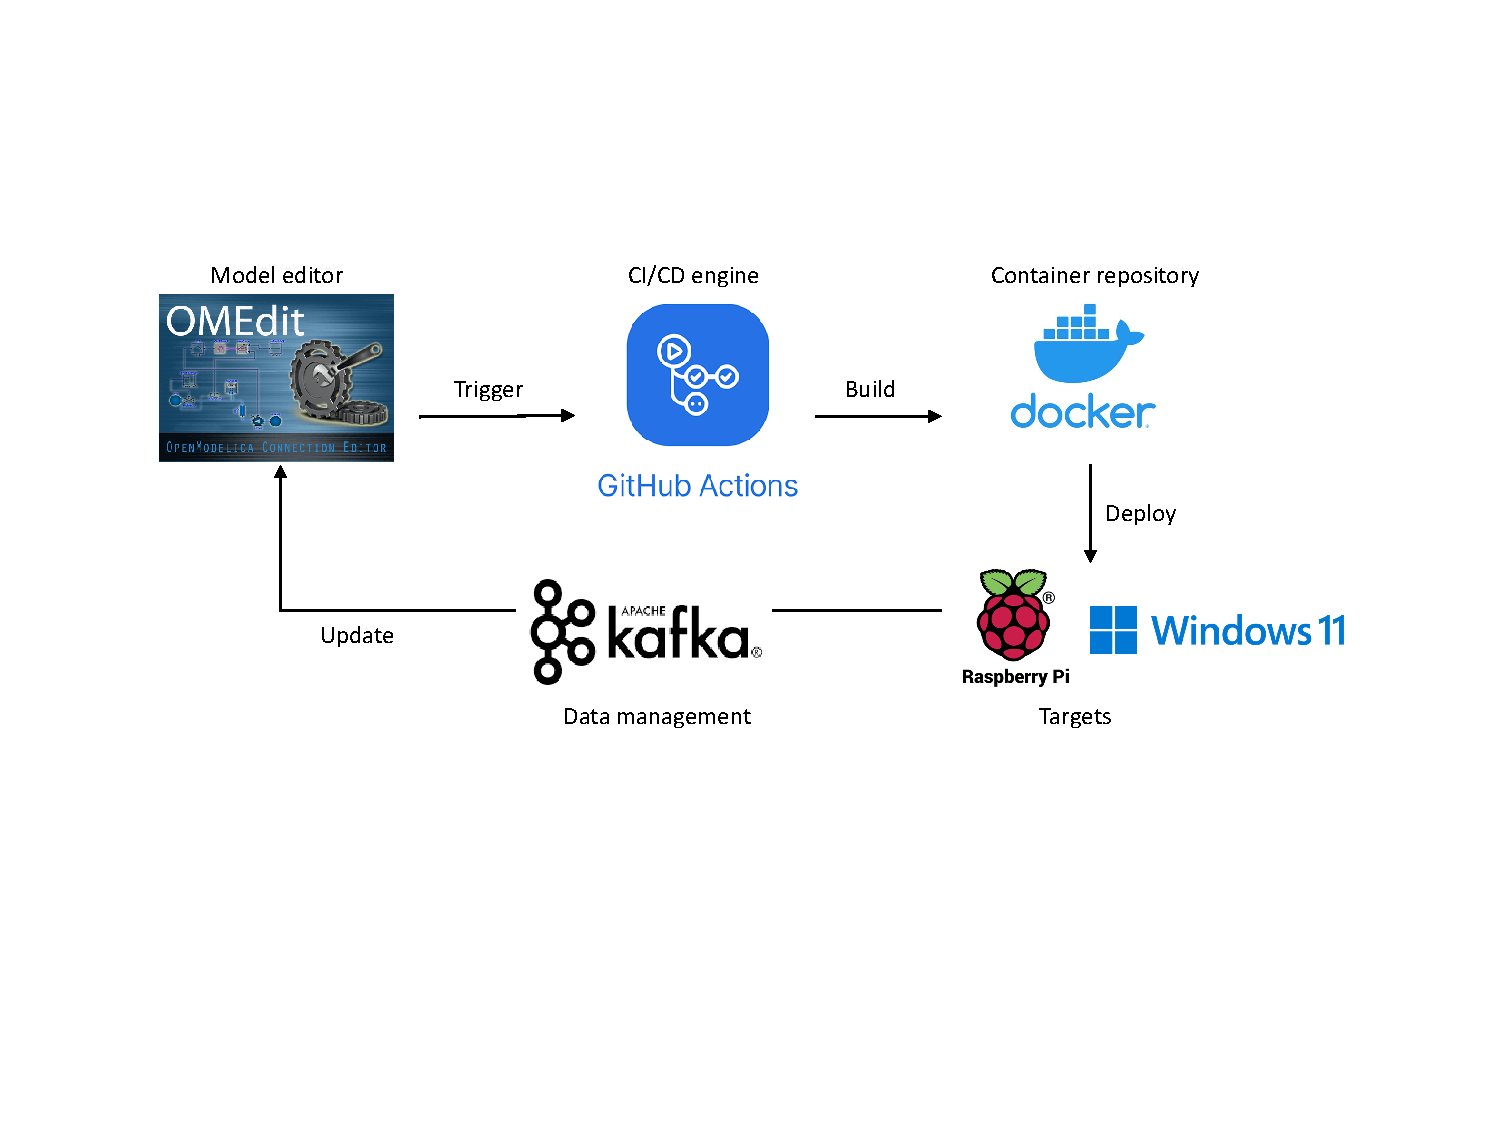
\includegraphics[scale=0.6]{figures/s1_twop_workflow.pdf}
  \caption{TwinOps implementation workflow for S1}
  \label{fig:s1_twop_workflow}
\end{figure}

For the \textit{model editor} stage, OMEdit \cite{OMEdit} is chosen to achieve the task. It is a graphical editing tool that allows user to connect individual FMUs to each other, and then export the topology to the System Structure and Parameterization (SSP) format \cite{SSP}. SSP is an open standard used to describe the port connections of a set of FMUs. It was created by the same organization which initiated the FMI standard, the Modelica Association. It is supported by an increasing number of major simulation environments which also support FMI. Figure \ref{fig:s1_twop_omedit} shows the layout of our use case in OMEdit.

\begin{figure}[hbt!]
  \centering
  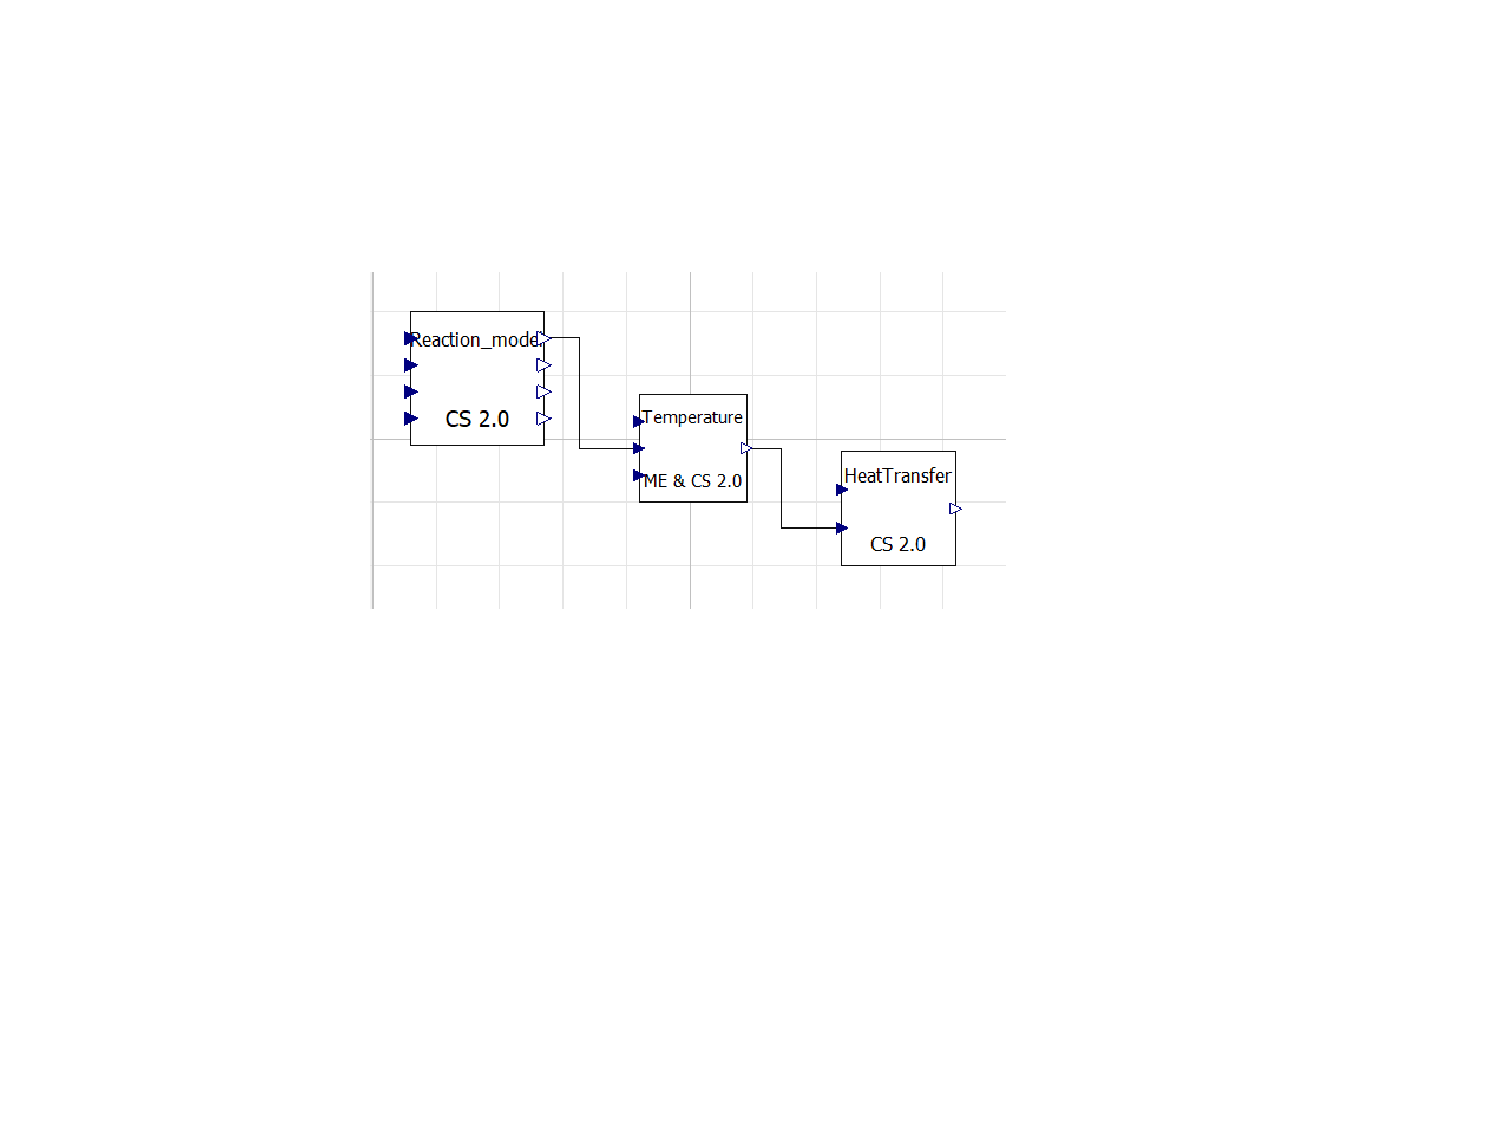
\includegraphics[scale=0.6]{figures/s1_twop_omedit.pdf}
  \caption[The SSP file rendered in OMEdit]{The SSP file rendered in OMEdit. Due to their different sources of origin, each FMU has varying supports for simulation modes, such as co-simulation version 2.0 (CS 2.0) or model exchange (ME). The FMUs also have different numbers of I/O ports. Since the models are designed to be``future-proof" for subsequent services, this is the reason why many I/O ports appear unused as they are irrelevant to this specific service}
  \label{fig:s1_twop_omedit}
\end{figure}

We choose GitHub Actions \cite{GitHubActions} as our \textit{CI/CD engine} for its native support for a vast variety of operating systems and programming frameworks. The operator can configure the pipeline using YAML---a human-readable data-serialization language that is commonly used for writing configuration files. 

As shown in Figure \ref{fig:s1_twop_cicd}, two phases (referred as jobs) are created in the pipeline, the left job represents CI, and the right job represents CD which will only be invoked if the CI job has succeeded. In the CI job, the SSP file is validated with the monitoring data which has been retrieved from a user-created trigger which activates every time new data are detected. The results will be saved as a GitHub Actions artifact. In the CD job, the task is to build and push the container image in Docker format \cite{Docker}.

\begin{figure}[hbt!]
  \centering
  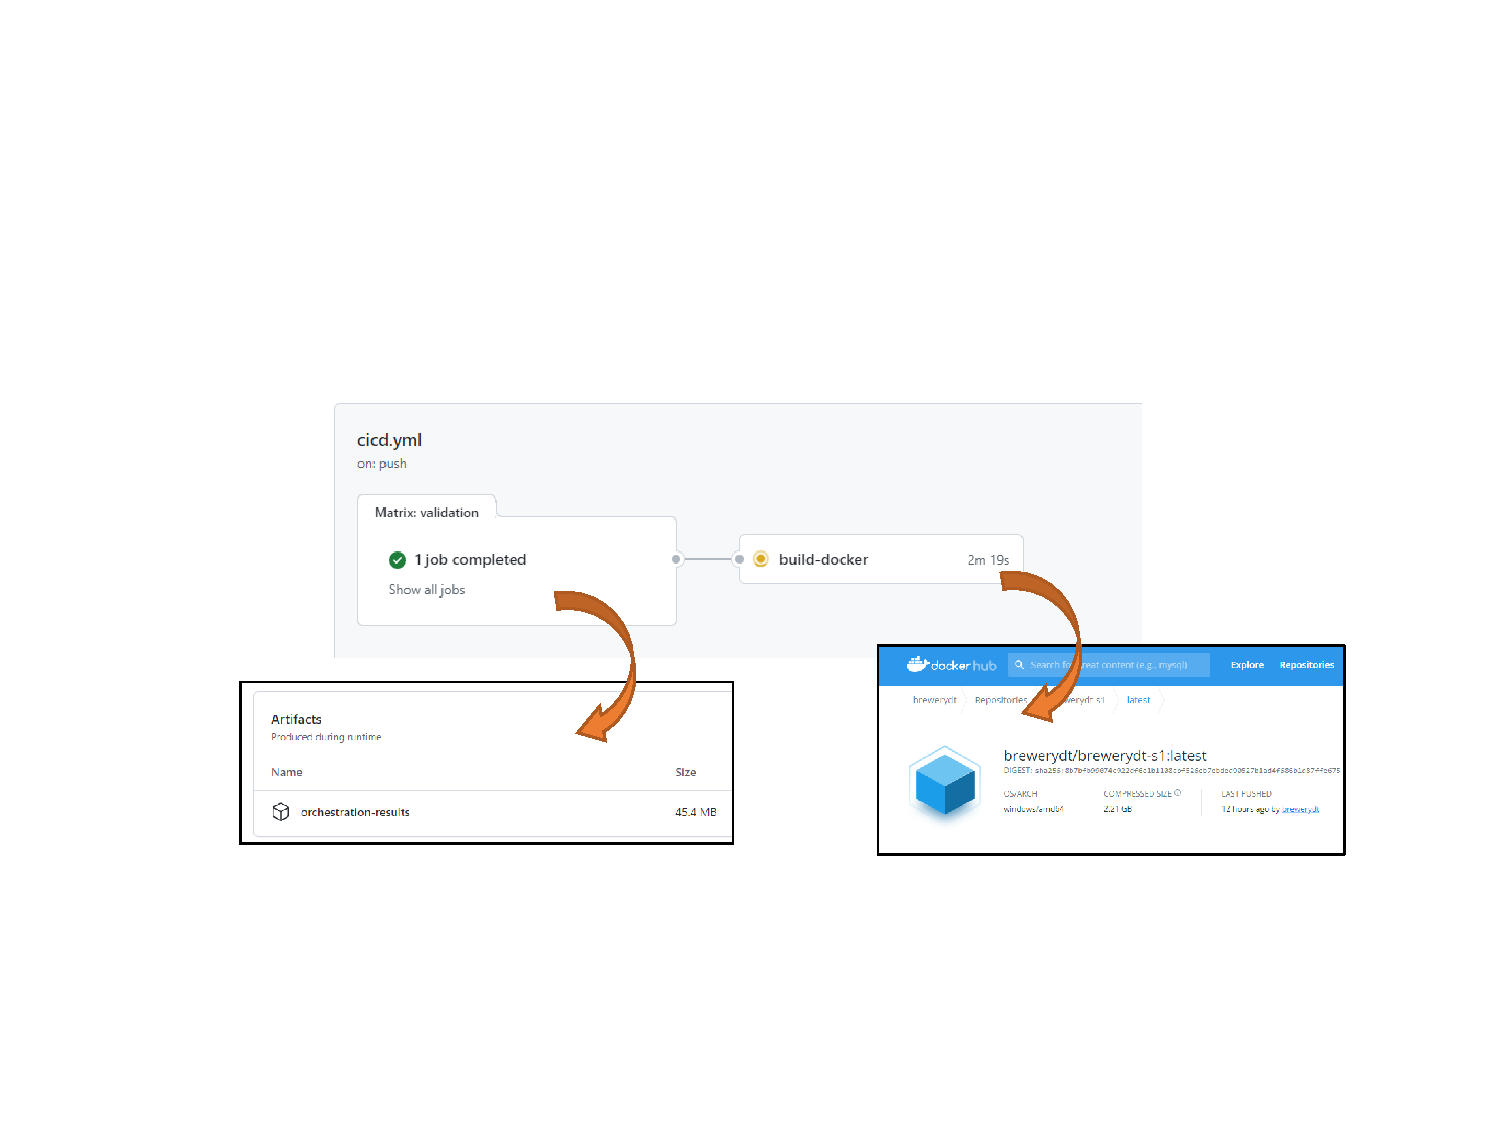
\includegraphics[scale=0.65]{figures/s1_twop_cicd.pdf}
  \caption{The CI (left) and CD (right) jobs and their outputs}
  \label{fig:s1_twop_cicd}
\end{figure}

The \textit{targets} for our use case are Raspberry Pi and Windows PC. The former is used as a data aggregation hub for all the sensor controls, and the latter is where we host our VE models.

One might notice the Kafka \cite{Kafka} block was not originally present in Subsection \ref{sec:selframe_twop} as a workflow stage. The reason being, the update path from the \textit{targets} to the \textit{model editor} stage could range from simplistic to rather complex, depending on the actual building blocks applied. In our use case, the \textit{targets} involve two different platforms---a microprocessor and a PC, leading us to introduce Kafka as an auxiliary tool to simplify the data management. In the DT context, models may access and store data in different formats and frequency. We adopt Kafka over the more traditional database due to its advantages of compartmentalized data queue and its active data streaming API. One can read more about the principles of Kafka in Appendix \ref{apd:kafka}.

\subsection{S1 in ThingsBoard}
Figure \ref{fig:s1_tb_entity} shows all the \textit{device} entities (sensors) and the \textit{asset} entities used in \textbf{S1}. The entities can be added by the operator manually in ThingsBoard UI, or be provisioned in bulk using CSV file. If multiple devices share the common settings, then one might consider creating ``device profiles" to improve entity management, like the ``Sensors" profile or the ``Models" profile shown in the figure. 

The asset named ``DT-PE" has a ``contain" \textit{relation} to all devices of the ``Sensors" profile. In other words, ``DT-PE" is an amalgamation of devices of the sensor type. The \textit{relation} defines a namespace which the \textit{rule chain} will adhere to.

\begin{figure}[hbt!]
  \centering
  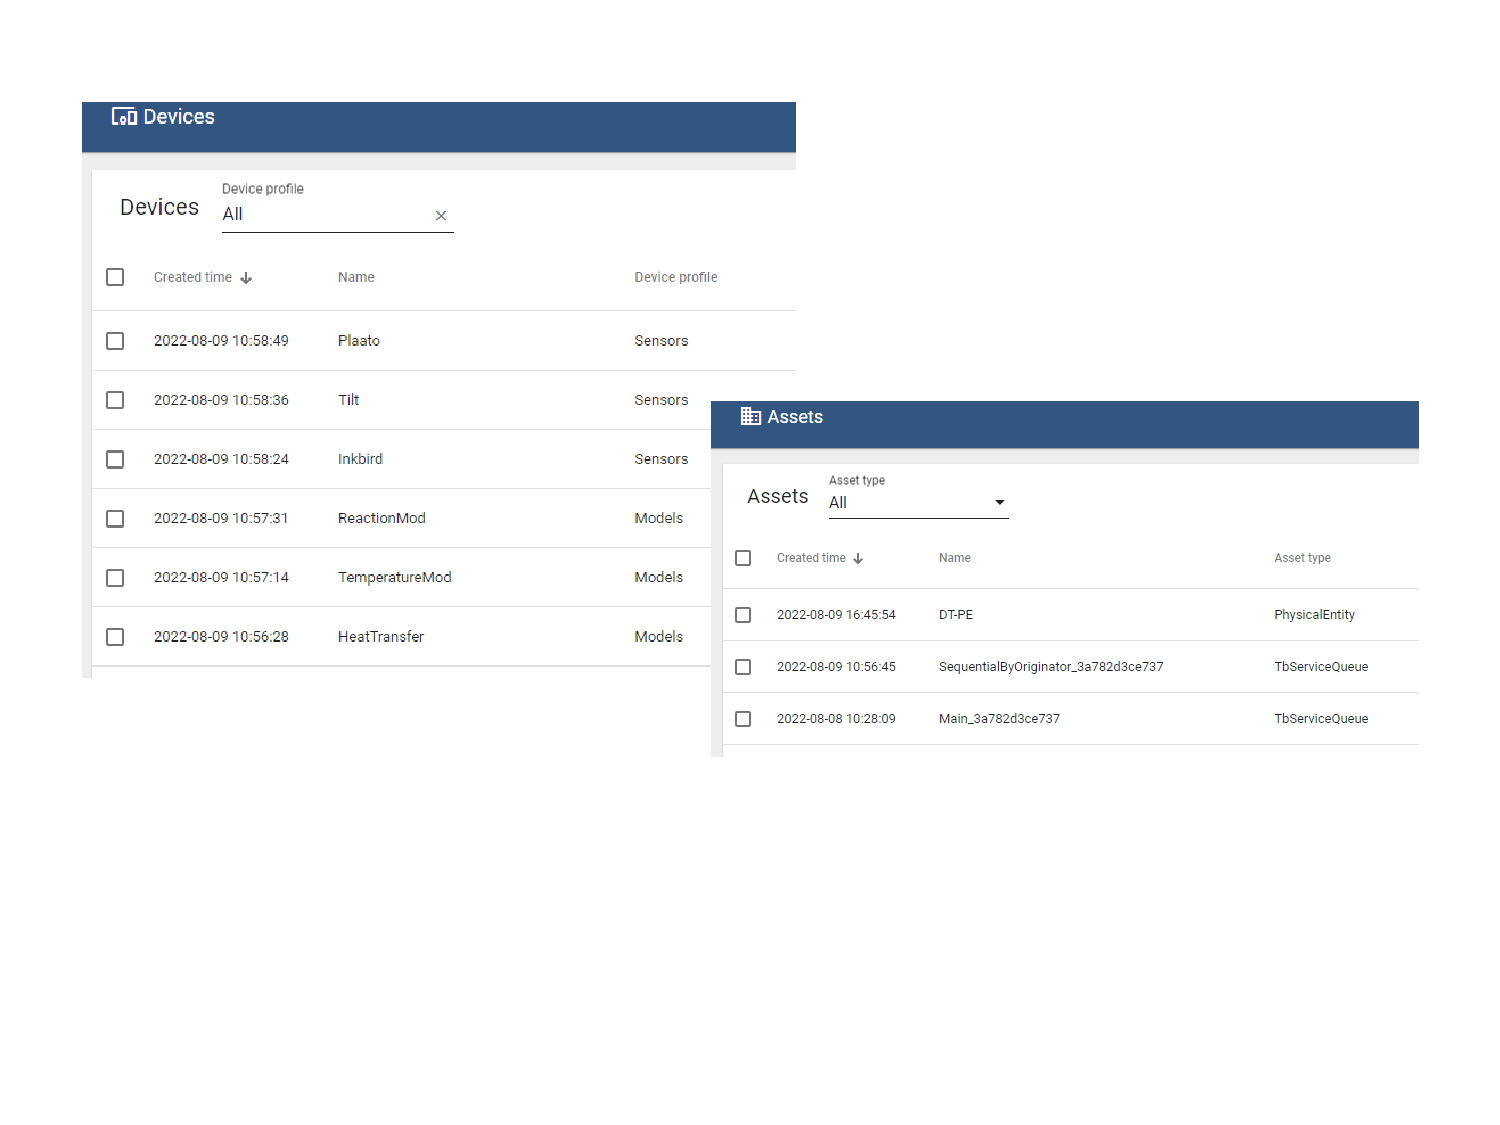
\includegraphics[scale=0.6]{figures/s1_tb_entity.pdf}
  \caption[S1 entity management in ThingsBoard]{S1 entity management in ThingsBoard. \texttt{Plaato} is the sensor used for collecting multitude of fermenter statuses; \texttt{Tilt} is a gravity detector; \texttt{Inkbird} is an ambient thermostat. The asset type \texttt{TbServiceQueue} is auto-generated  by the core process to handle network traffics.}
  \label{fig:s1_tb_entity}
\end{figure}

\begin{figure}[hbt!]
  \centering
  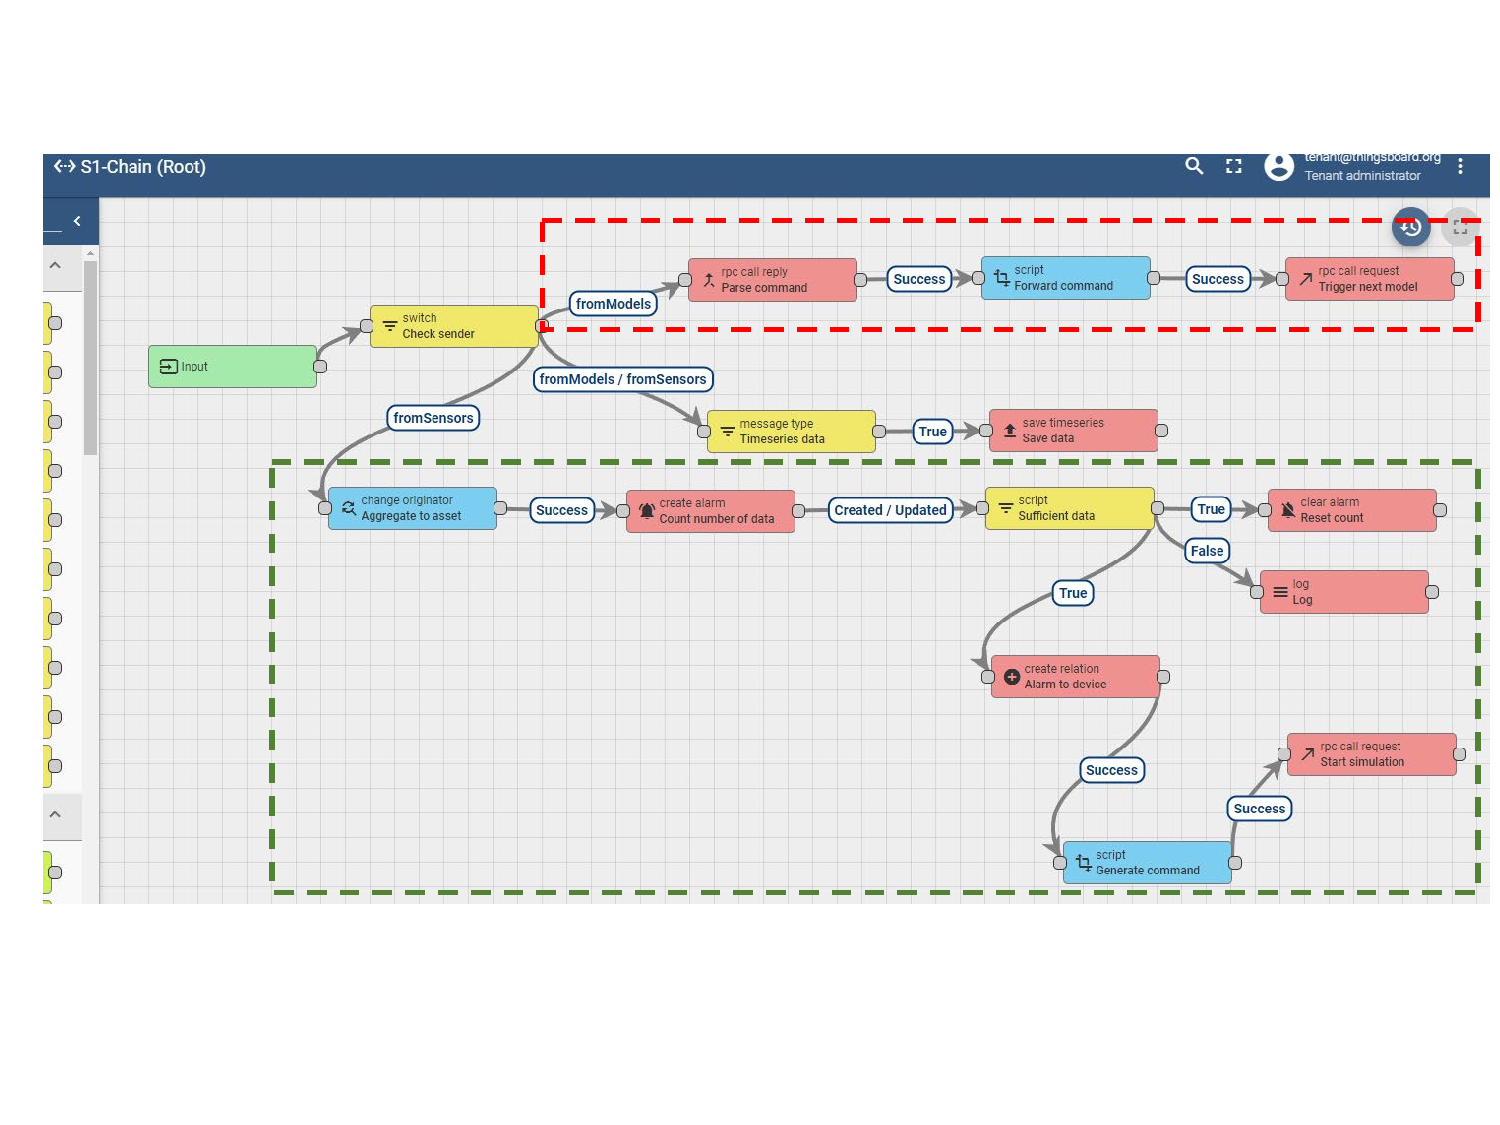
\includegraphics[scale=0.6]{figures/s1_tb_rulechain.pdf}
  \caption{S1 rule chain in ThingsbBoard}
  \label{fig:s1_tb_rulechain}
\end{figure}

Figure \ref{fig:s1_tb_rulechain} presents the \textit{rule chain}, which has three major parts:
\begin{itemize}
\item The top branch (red dashed border) is the event-based logic for inter-models procedure calls. Its primary function is to orchestrate by signaling from the originator model to the destination model, such that a correct execution sequence could be maintained. 
\item The bottom branch (green dashed border) is for updating the monitoring data from the sensors to the model states. The ``DT-PE" asset plays an important role here for transforming the local namespace of the sensor data into the global namespace of the DT, such that the models can use the data without binding to specific sensor devices.
\item The nodes in the middle are responsible for recording and saving data with timestamps for future usage by the real-time dashboard. 
\end{itemize}

\begin{figure}[hbt!]
  \centering
  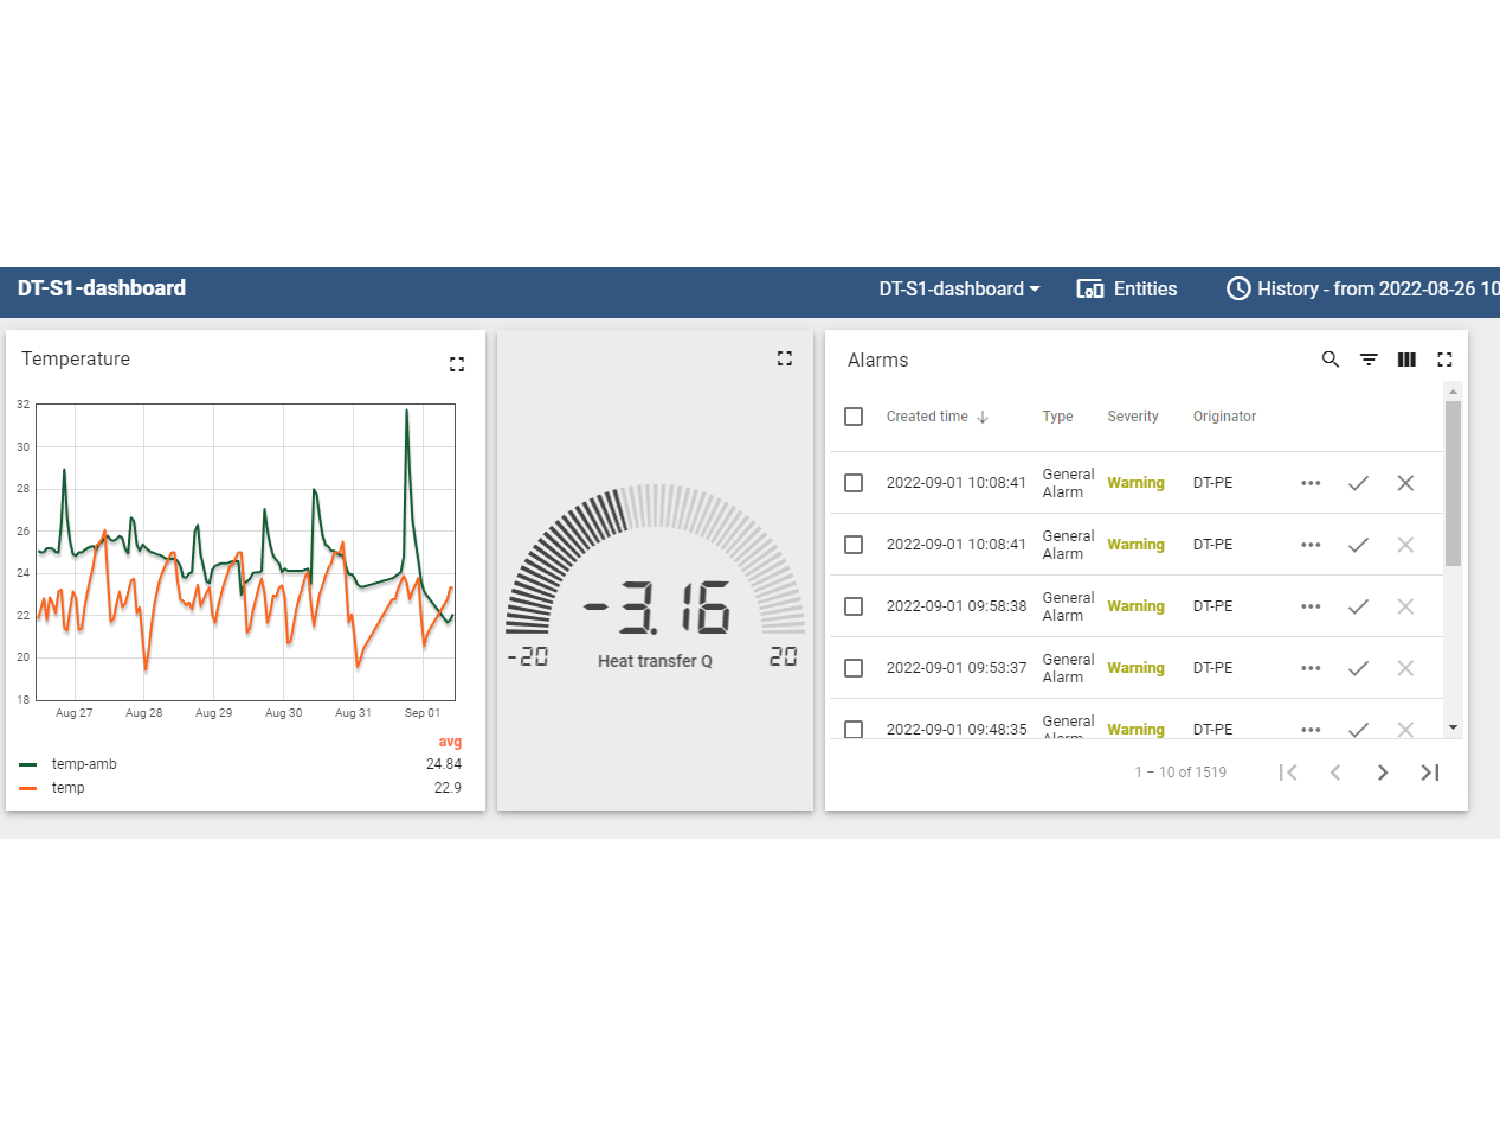
\includegraphics[scale=0.5]{figures/s1_tb_dashboard.pdf}
  \caption{A snapshot of the real-time dashboard in ThingsBoard for the \textit{heat transfer model}}
  \label{fig:s1_tb_dashboard}
\end{figure}

As introduced in Subsection \ref{sec:selframe_tb}, the real-time dashboard offers a wide range of \textit{widgets} for the operator to incorporate the human-in-the-loop concept to DT operations. In Figure \ref{fig:s1_tb_dashboard} we demonstrate the usage of built-in \textit{widgets} that visualize the system information. The plot on the left records the temperatures monitored from the PEs. The middle gauge displays the heat loss prediction at a given future moment. The alarm widget on the right side notifies the operator every time the \textit{heat transfer model} has been updated.

\subsection{S1 in Ptolemy II} \label{sec:s1demopt2}

\begin{figure}[hbt!]
  \centering
  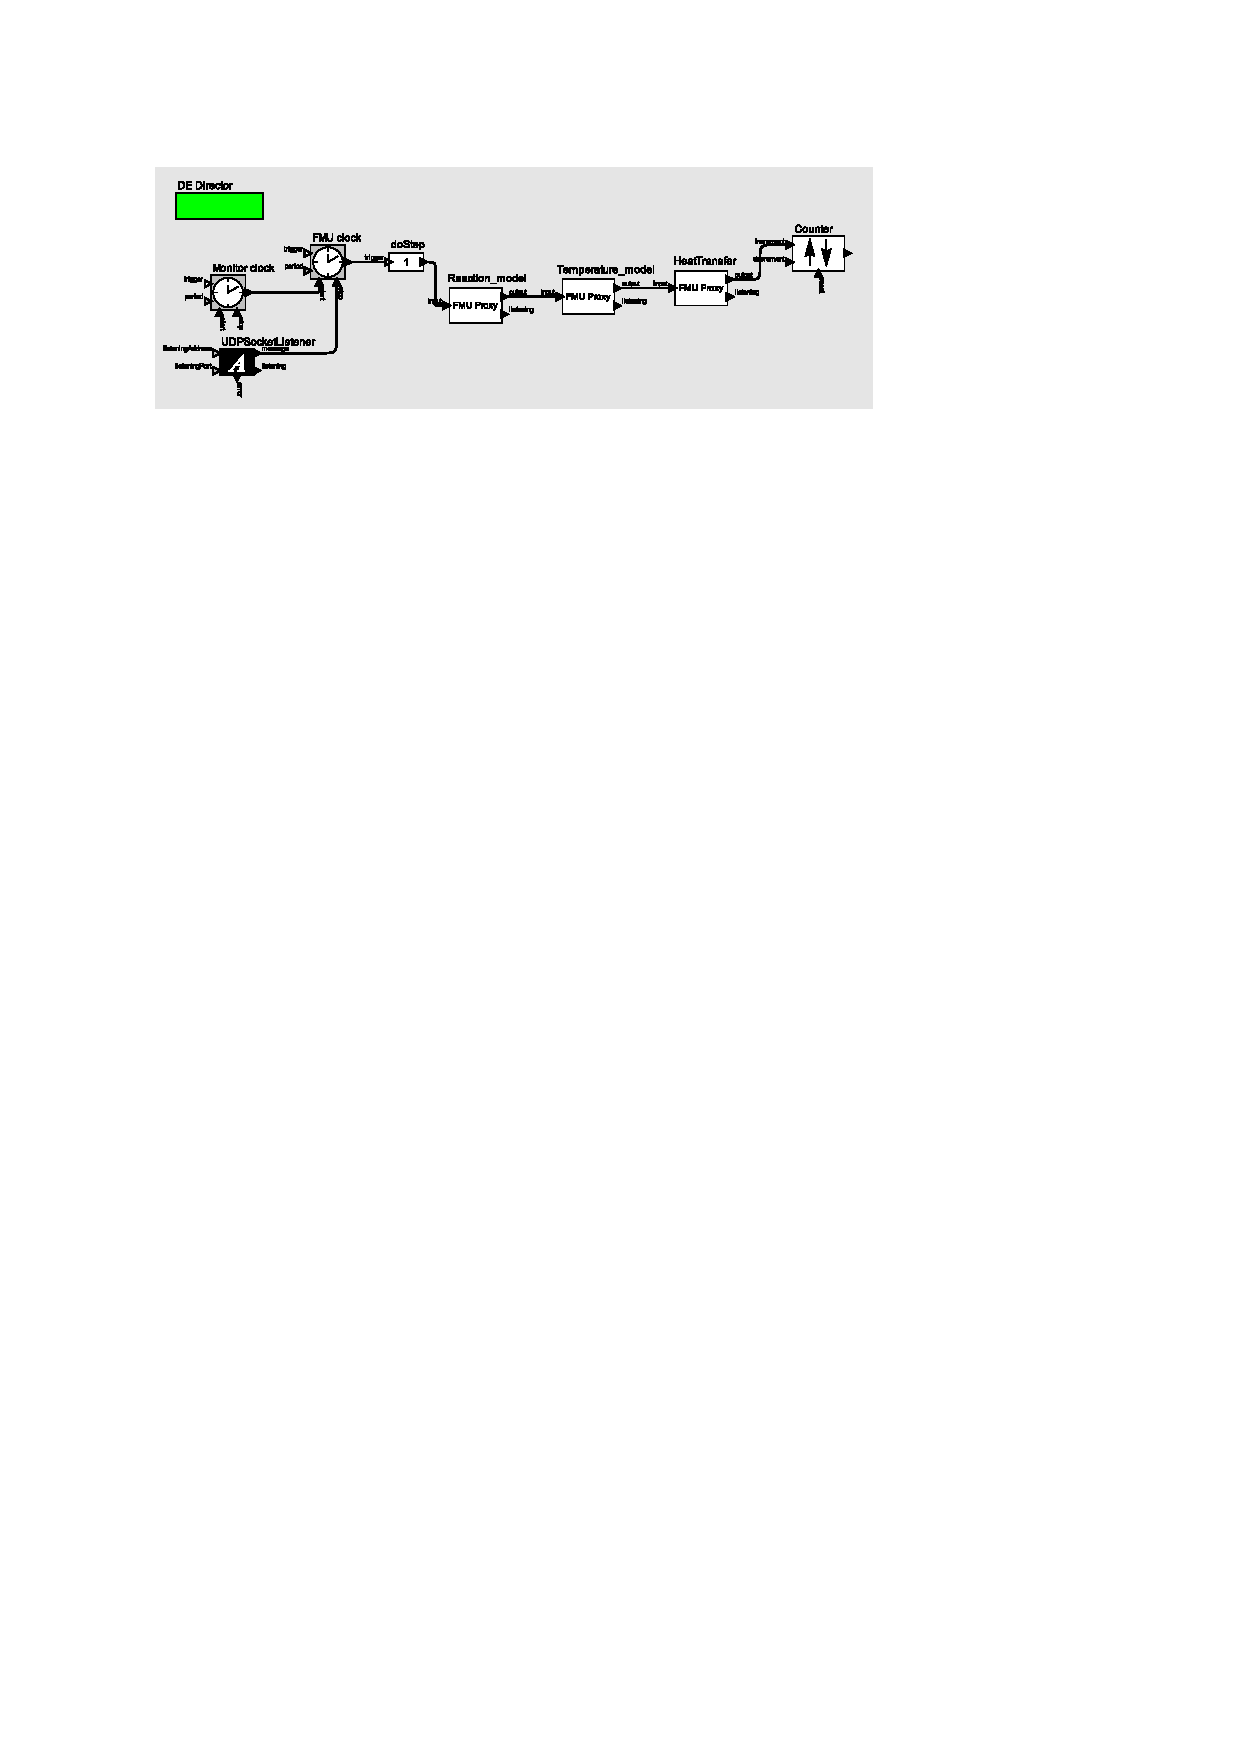
\includegraphics[scale=1.1]{figures/s1_pt_de.pdf}
  \caption{Ptolemy II design for S1}
  \label{fig:s1_pt_de}
\end{figure}

Figure \ref{fig:s1_pt_de} displays the overall design of \textbf{S1}. The Discrete Event (DE) \texttt{Director} is used as the orchestrating instructions are treated as individual ``events". There are two clock sources, \texttt{Monitor clock} is synchronized against real-world time such that it takes up the task to trigger the models based on the sensor events of PEs. On the other hand, \texttt{FMU clock} dictates the time advancement of the FMU models. It is initialized---by \texttt{Monitor clock}---when the monitoring data are ready, and is terminated when all models have completed simulations---notified via a dedicated UDP listener. Each \texttt{FMU Proxy} represents a model of the VEs.

Since Ptolemy II does not posses data management actors suitable for our DT, we utilize Kafka to fetch the monitoring data in order to update the models and to store the computed results.

Although Ptolemy II has built-in support for FMI by its \texttt{FMUImporter} actor, however, from our experiments we discover it has several weaknesses which lead to undesirable crashes (see Appendix \ref{apd:fmi} for details). As a circumvention, a user defined actor named \texttt{FMU Proxy} is created as shown in Figure \ref{fig:s1_pt_proxy}. The actor serves as a middle-man who forwards the orchestrating instructions from Ptolemy II to the solver outside of the environment via UDP sockets. Using this approach, the operator can orchestrate the FMU models as if they are inside the Ptolemy II environment.   

\begin{figure}[hbt!]
  \centering
  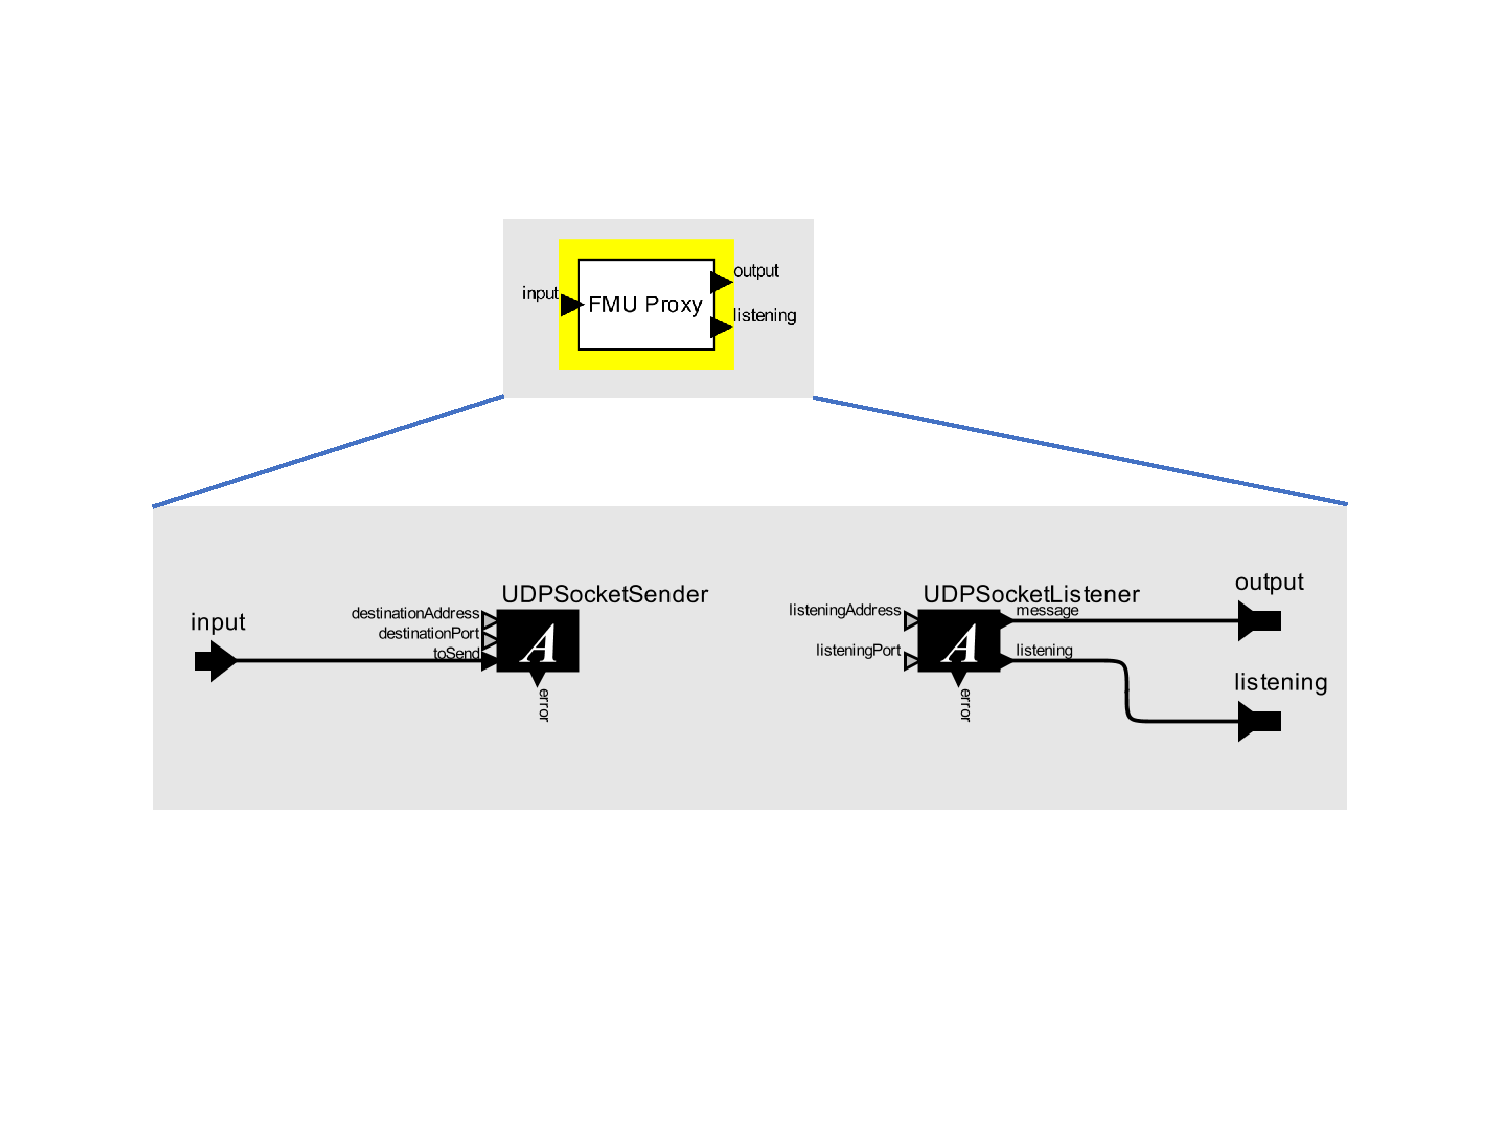
\includegraphics[scale=0.45]{figures/s1_pt_proxy.pdf}
  \caption{The internal implementation of \texttt{FMU Proxy}}
  \label{fig:s1_pt_proxy}
\end{figure}

\section{Production Control (S2) demonstrations}\label{sec:s2demo}
In \textbf{S2}, the control model generates a command based on the fed data. Then the commands are sent from the VE to the actuator---a water pump controller---of the PE. Most of the framework infrastructures are inherited from \textbf{S1}. As more services are introduced, we start to benefit from the dividends of frameworks in term of a significant reduction in developer's workload. 

An alternative implementation that uses human-in-the-loop control scheme instead of fully automated decisions can be found in Appendix \ref{apd:humanloop}. The alternative demonstrates how DTs can be used to assist the operators in a scenario where human intervention is necessary.  
  
\subsection{S2 in TwinOps} 
On top of the existing \textbf{S1} workflow, the operator can simply add the new model to the SSP file as in Figure \ref{fig:s2_twop_omedit}. After that, a new task needs to be added to the CI/CD pipeline so as to pass the computed commands to a remote webhook that controls the water pump.

\begin{figure}[hbt!]
  \centering
  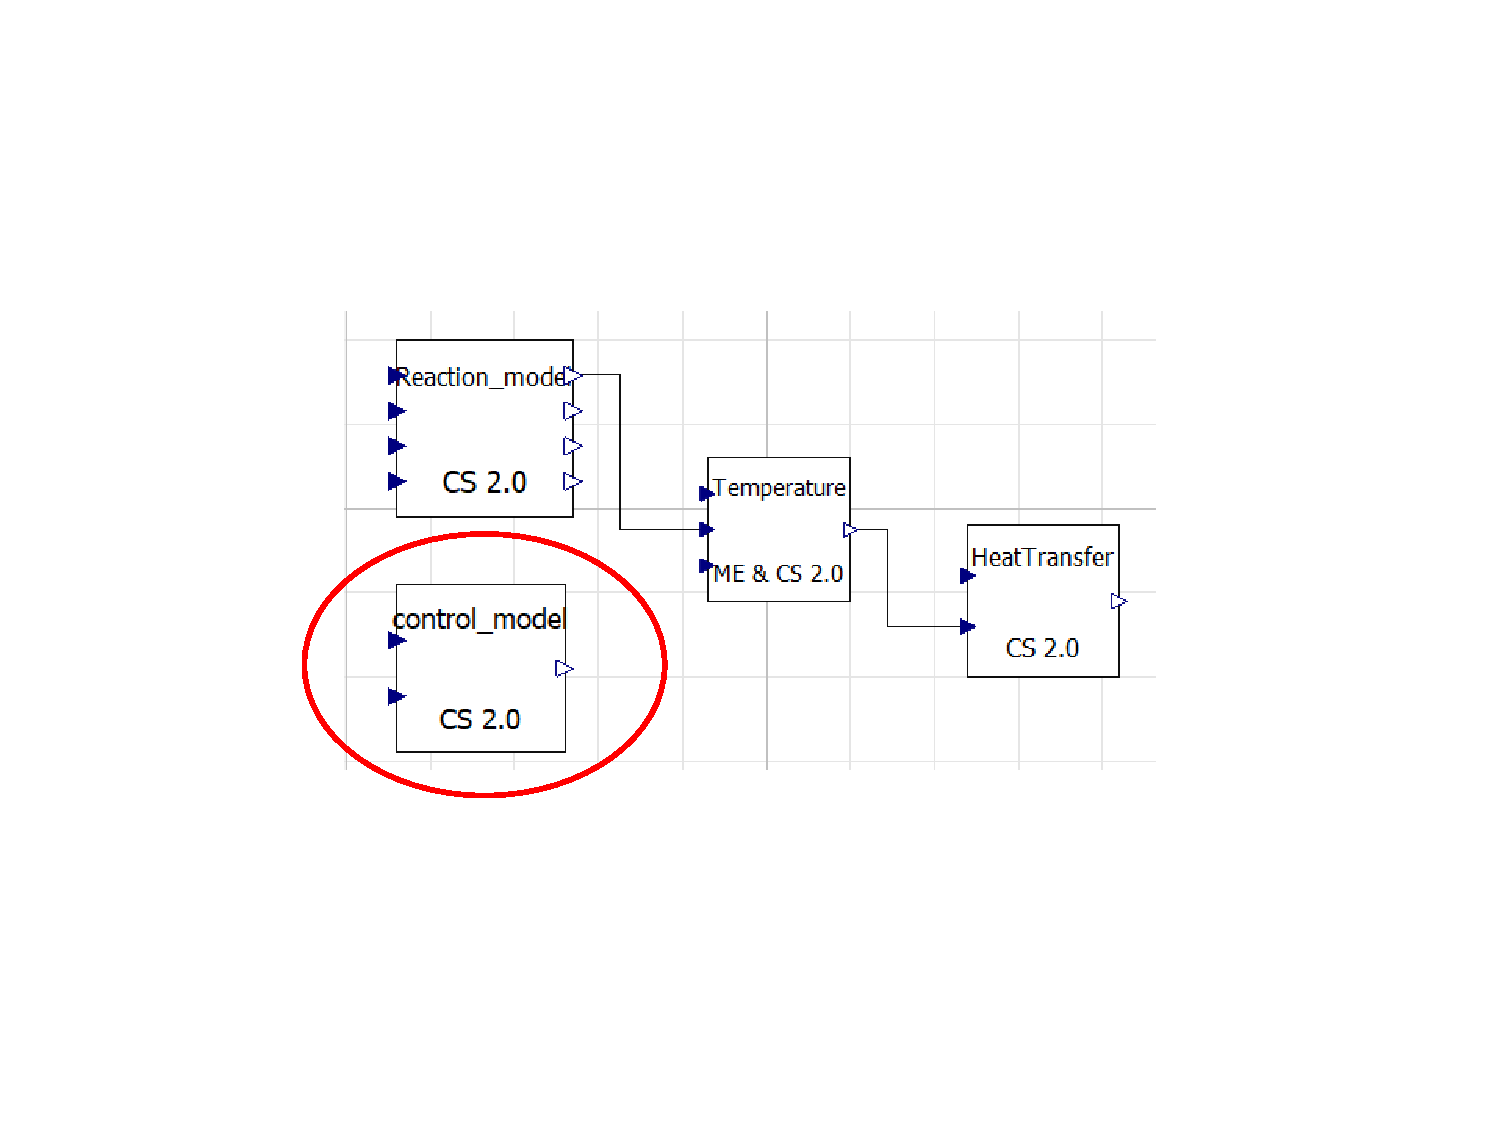
\includegraphics[scale=0.4]{figures/s2_twop_omedit.pdf}
  \caption{The SSP layout of S2}
  \label{fig:s2_twop_omedit}
\end{figure}

\subsection{S2 in ThingsBoard} 
The control model is provisioned as an entity of the ``Models" type just as with the models in \textbf{S1} previously.

A new \textit{rule chain} shown in Figure \ref{fig:s2_tb_rulechain} is added to support the control service. The top branch is responsible for triggering the control model, similarly to the way of \textbf{S1}. The bottom branch takes care of sending the command message to the actuator. 

\begin{figure}[hbt!]
  \centering
  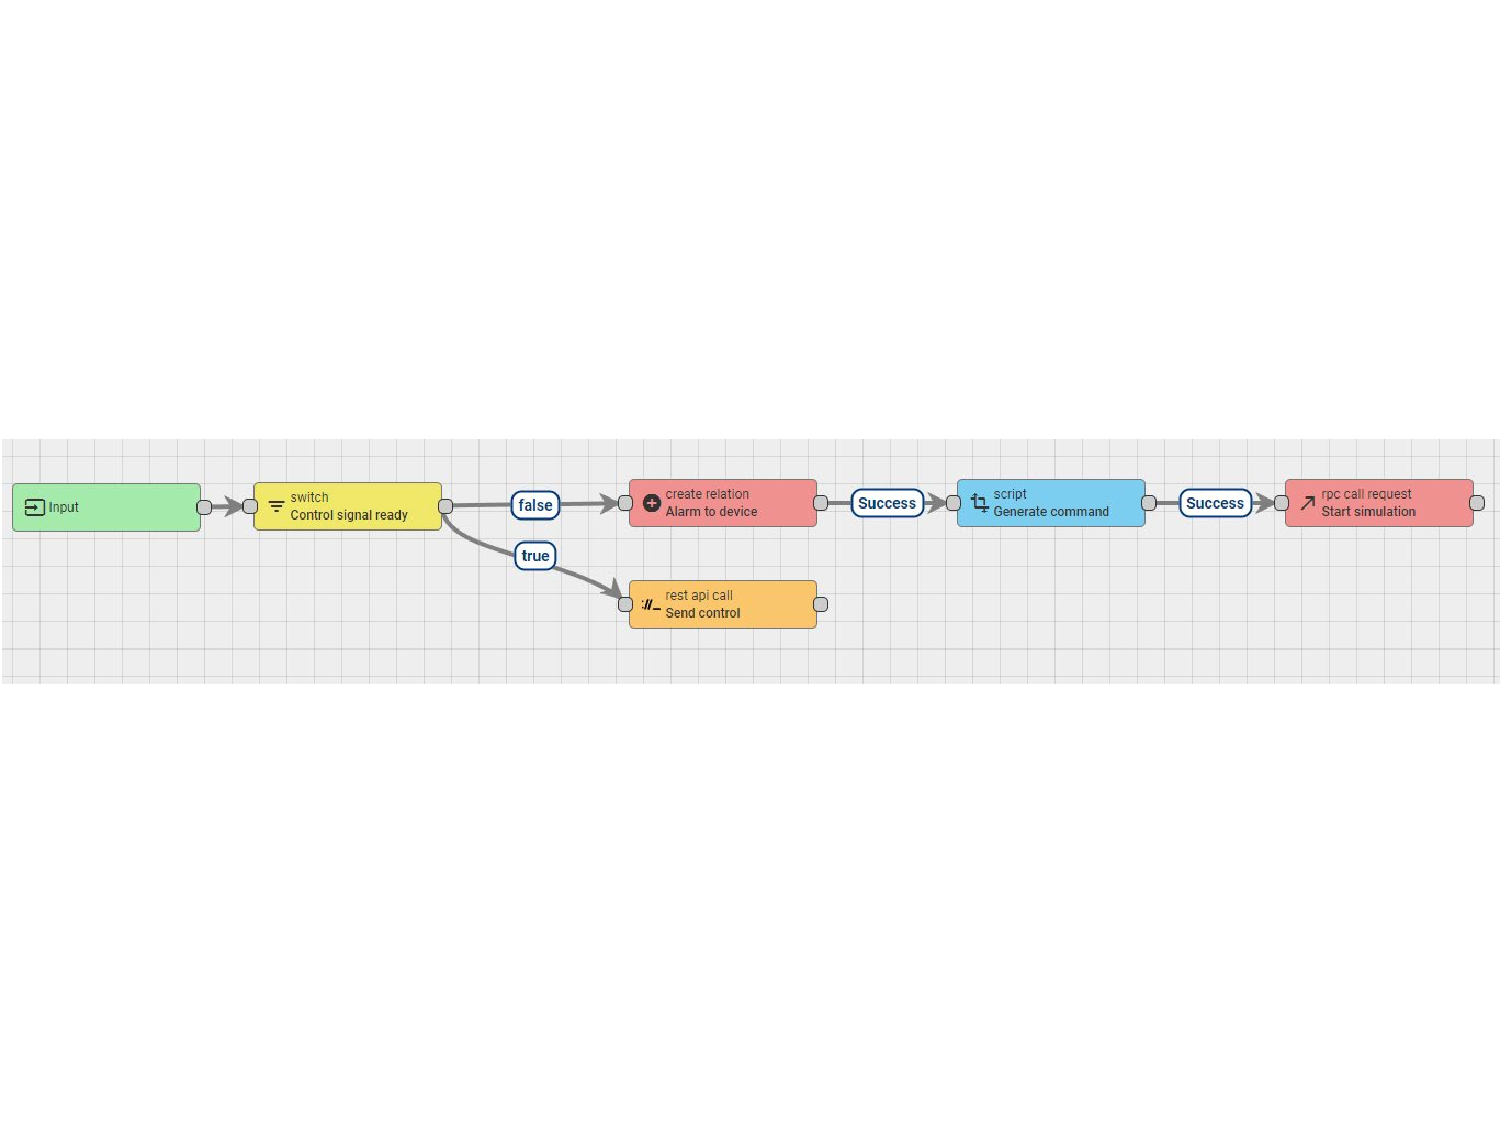
\includegraphics[scale=0.55]{figures/s2_tb_rulechain.pdf}
  \caption{S2 rule chain in ThingsBoard}
  \label{fig:s2_tb_rulechain}
\end{figure}

The \textbf{S2} \textit{rule chain} is connected to the ``root" \textit{rule chain} of \textbf{S1} via the ``Flow" type nodes (the purple color nodes in Figure \ref{fig:s2_tb_rulechain_root}), so the established data routing paths could be reused.

\begin{figure}[hbt!]
  \centering
  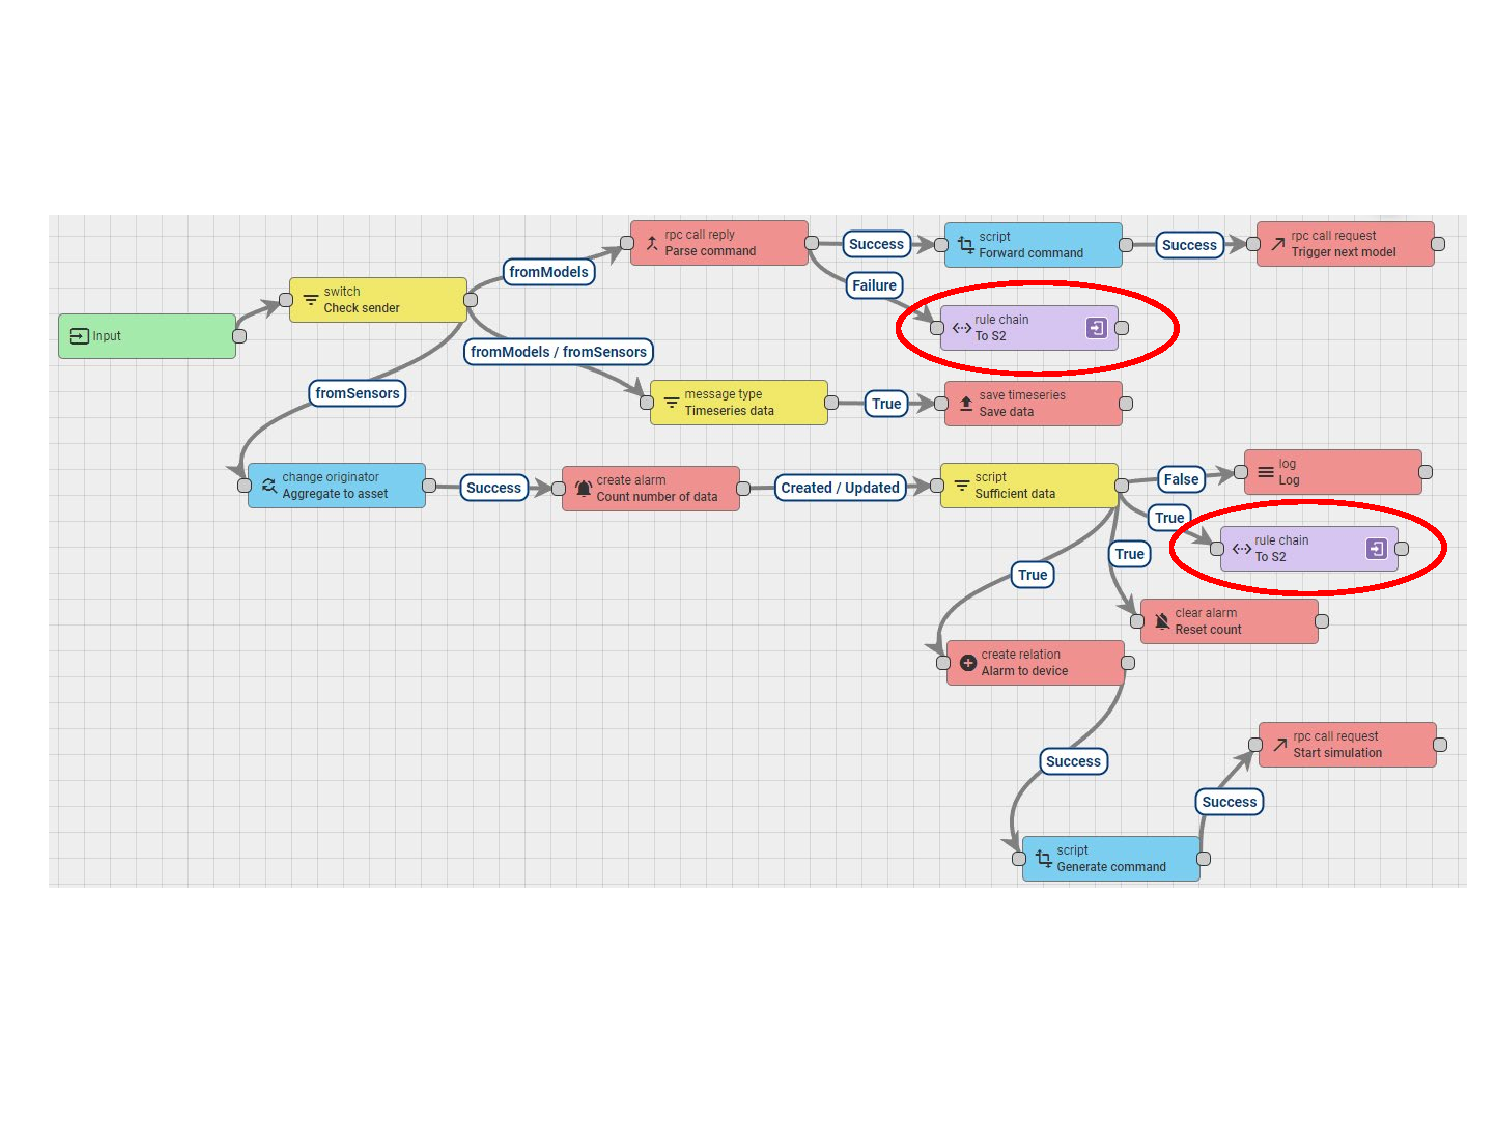
\includegraphics[scale=0.5]{figures/s2_tb_rulechain_root.pdf}
  \caption{Integration of S2 to the root rule chain}
  \label{fig:s2_tb_rulechain_root}
\end{figure}

In the real-time dashboard, the computed control signal are superimposed onto the timeseries chart of the temperatures, as shown in Figure \ref{fig:s2_tb_dashboard}. 

\begin{figure}[!htb]
  \centering
  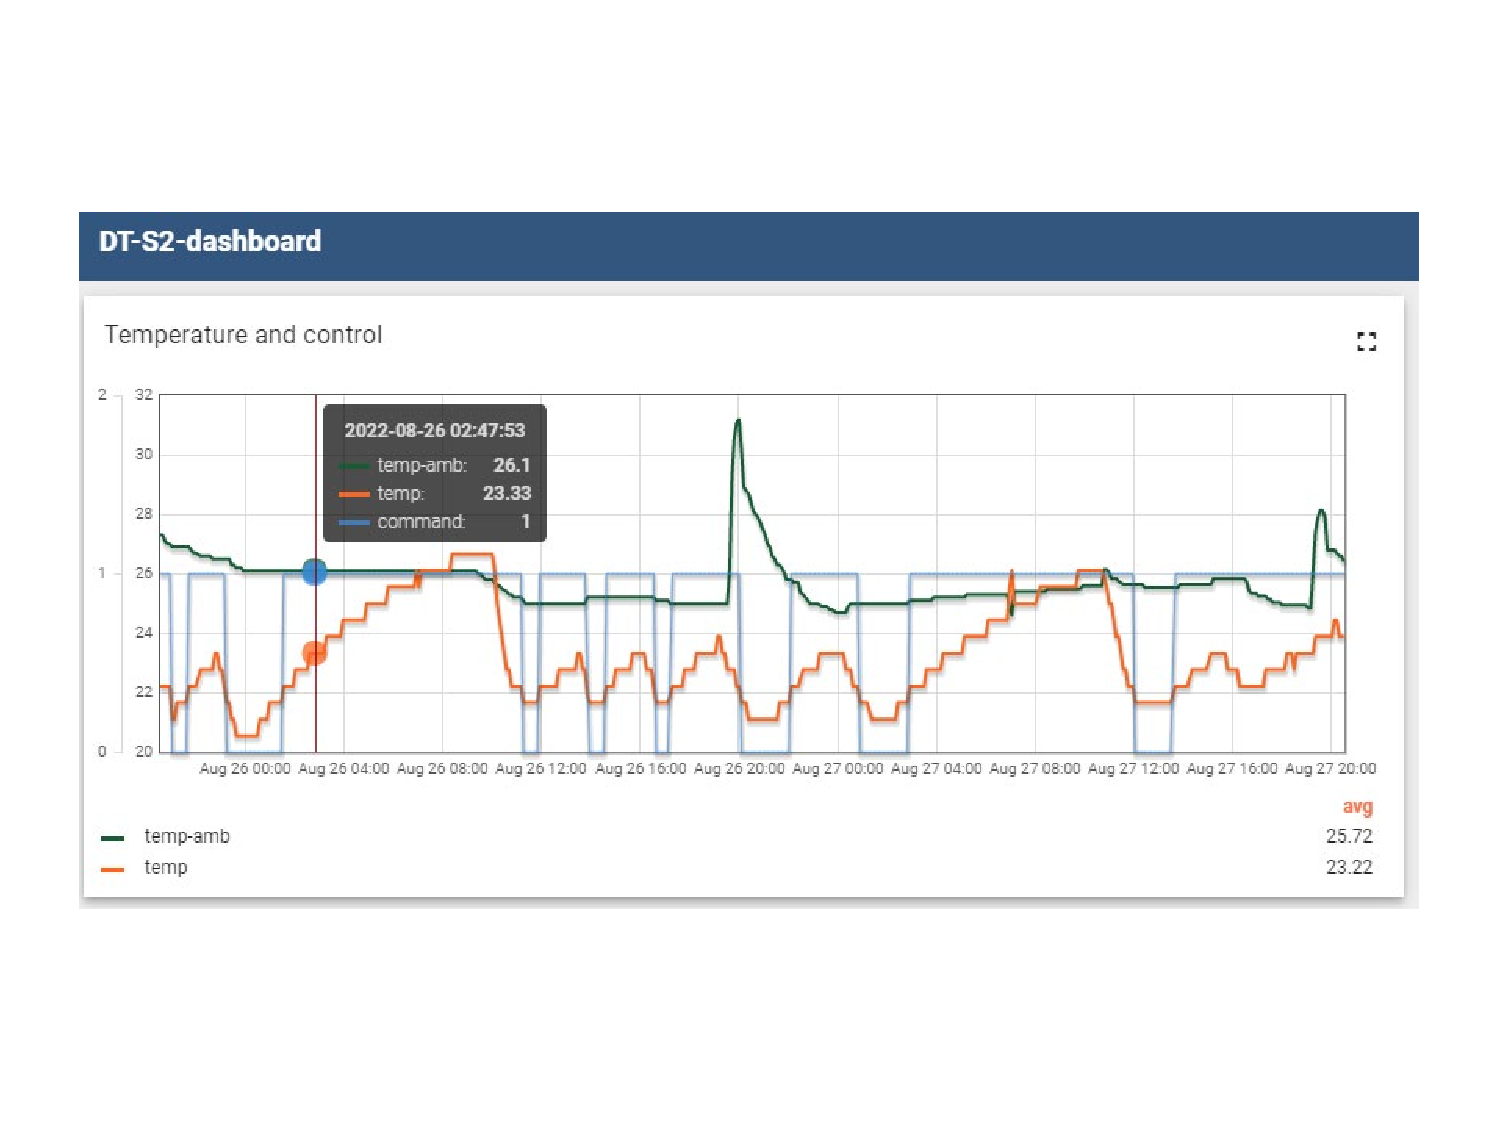
\includegraphics[scale=0.44]{figures/s2_tb_dashboard.pdf}
  \caption[A snapshot of S2 real-time dashboard]{A snapshot of S2 real-time dashboard. The chart displays the room temperature (green), the fermenter temperature (orange), and the output of the control model (blue).}
  \label{fig:s2_tb_dashboard}
\end{figure}

One can notice a pattern in which the ``high" (switch on) intervals of the control commands are followed by the climbing of the internal temperature, and vice versa. This example demonstrates how the framework can offer analytics that enable the operator to trace and assess the effects of the control system.
 
\subsection{S2 in Ptolemy II} 
Shown in Figure \ref{fig:s2_pt_composite}, we utilize the ``composite actor" (circled) in Ptolemy II to encapsulate \textbf{S2} and integrate it to the existing design of \textbf{S1}, more specifically, reusing the \texttt{clock} actors. Using composite actors improves the overall portability as the operator can attach new services to the root service (\textbf{S1}).

\begin{figure}[hbt!]
  \centering
  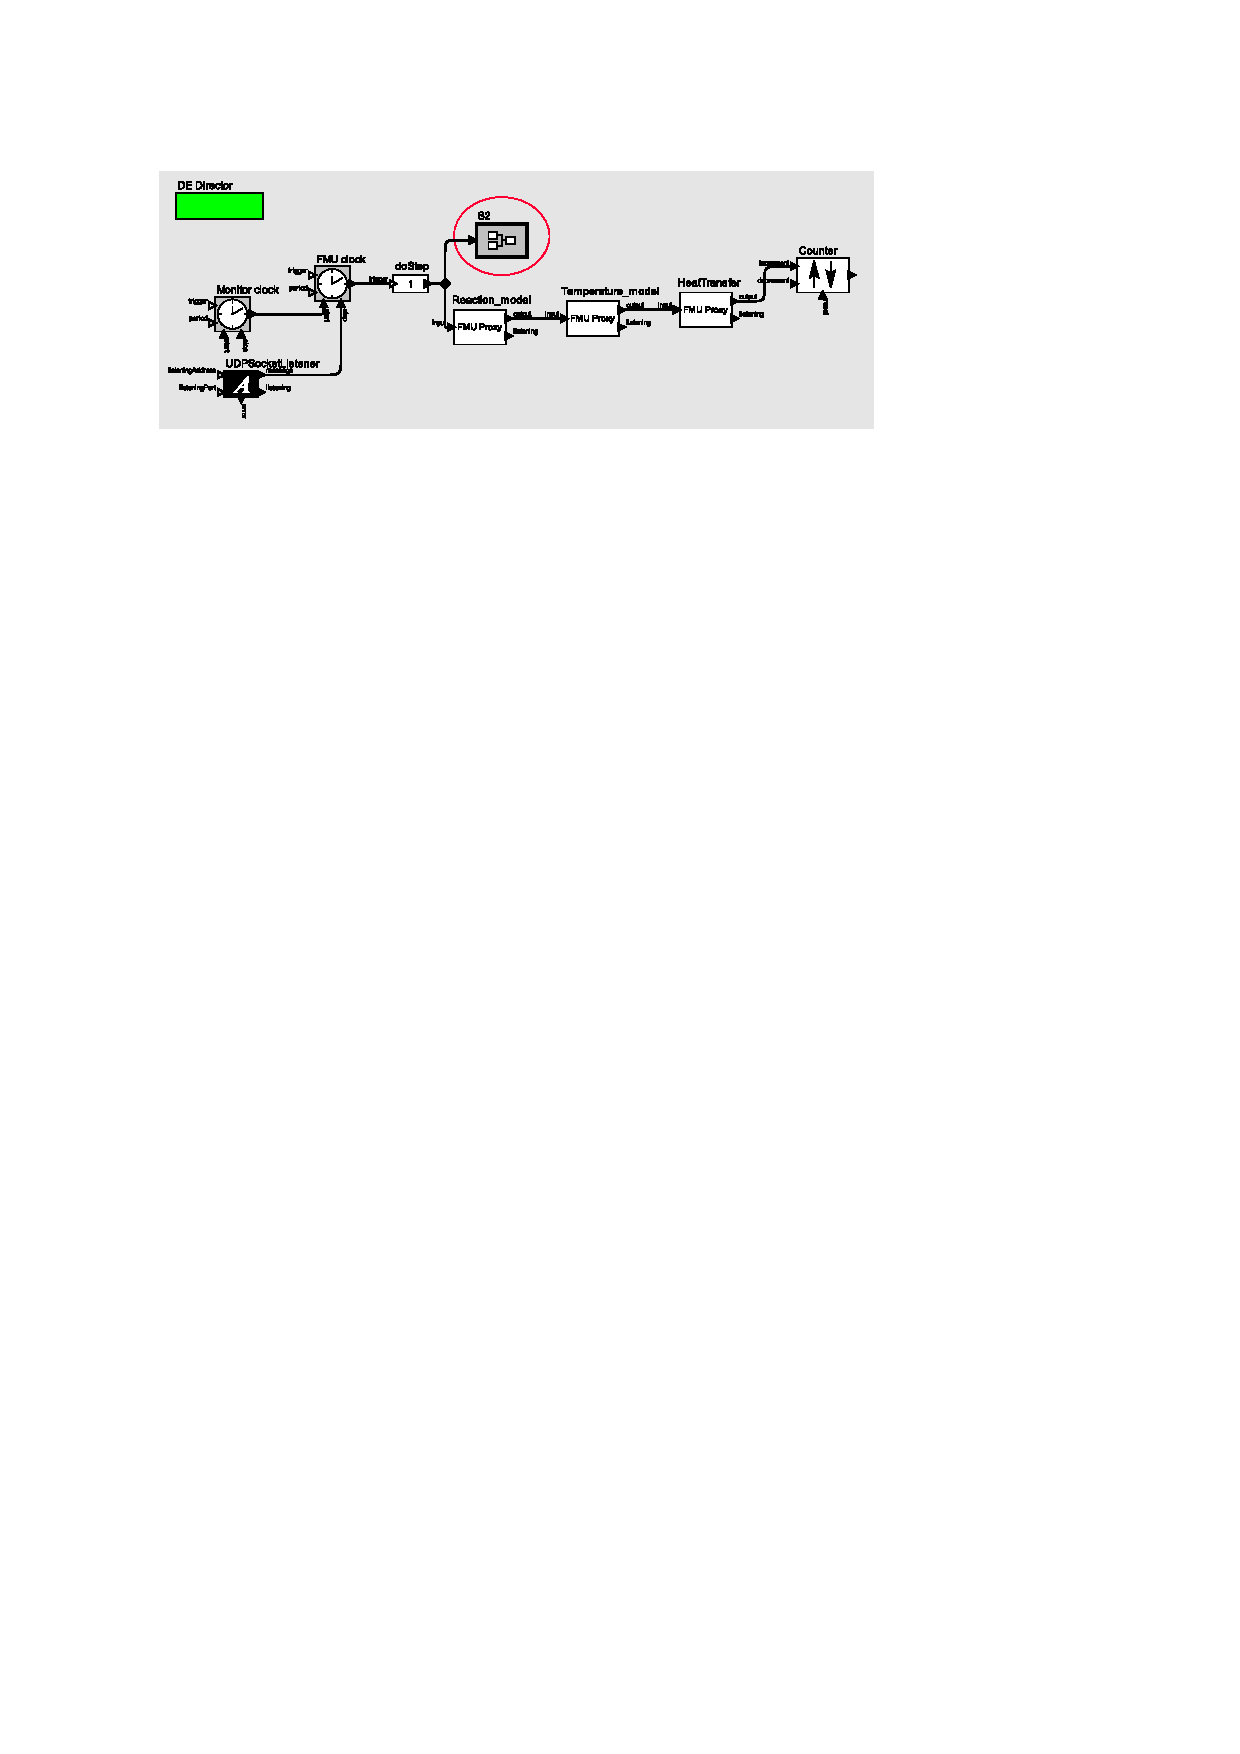
\includegraphics[scale=1.1]{figures/s2_pt_composite.pdf}
  \caption{The encapsulation of S2}
  \label{fig:s2_pt_composite}
\end{figure}

The internal implementation of \textbf{S2} is shown in Figure \ref{fig:s2_pt_internal}, where the \texttt{FMU Proxy} is triggered by the \texttt{FMU clock}---shared by \textbf{S1}---from the outside. Then the computed command is sent to a remote actuator webhook using the REST client actor.

\begin{figure}[hbt!]
  \centering
  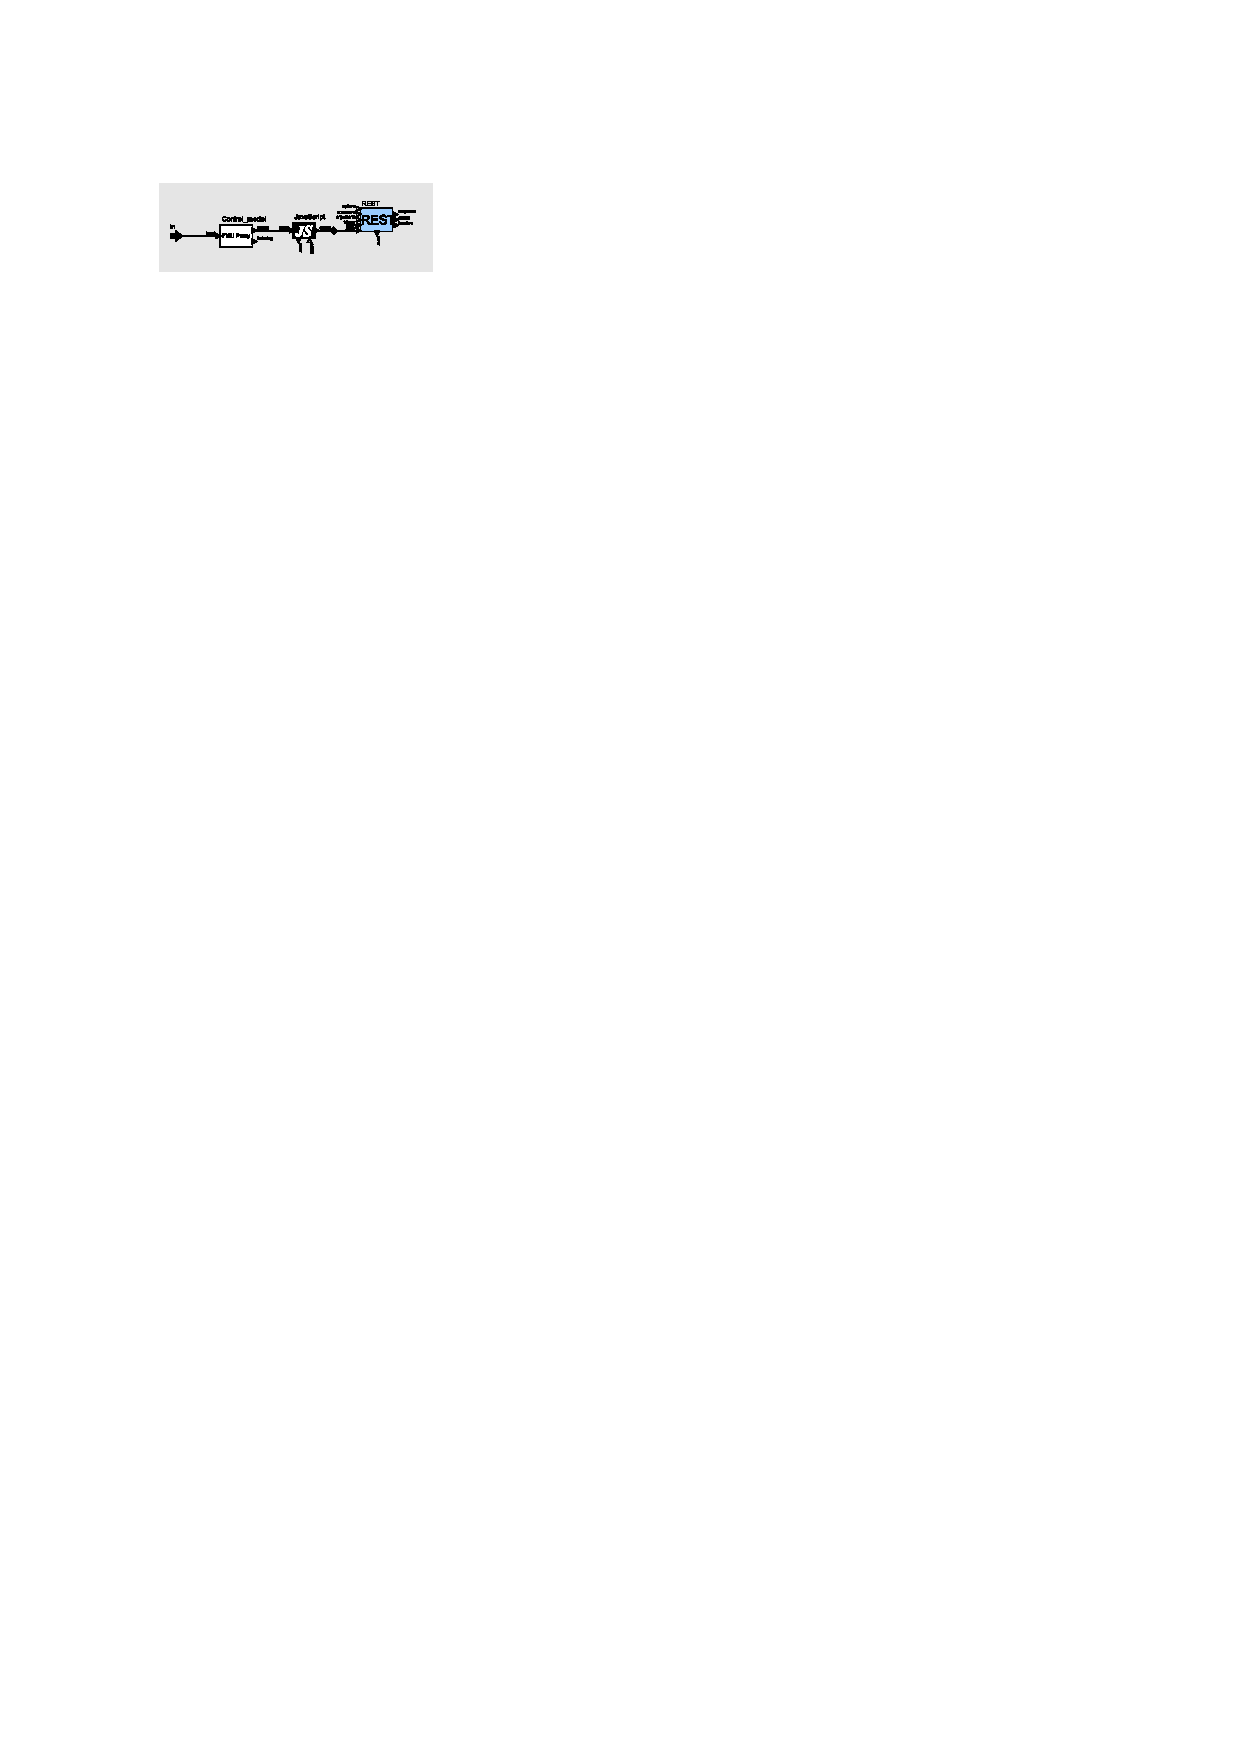
\includegraphics[scale=2.1]{figures/s2_pt_internal.pdf}
  \caption{S2 design in Ptolemy II}
  \label{fig:s2_pt_internal}
\end{figure}

We conclude the implementations for \textbf{S1} and \textbf{S2} here. In the next chapter we will compare the frameworks' characteristics, performances, and non-functional properties.
